\subsection{Goniometriche}
    \subsubsection{Seno e Coseno}
        Sia $U = \{(x,y) \in \mathbb{R}\ |\ x^{2} + y^{2} = 1\}$ la \textbf{circonferenze goniometrica}.\\
        \begin{center}
            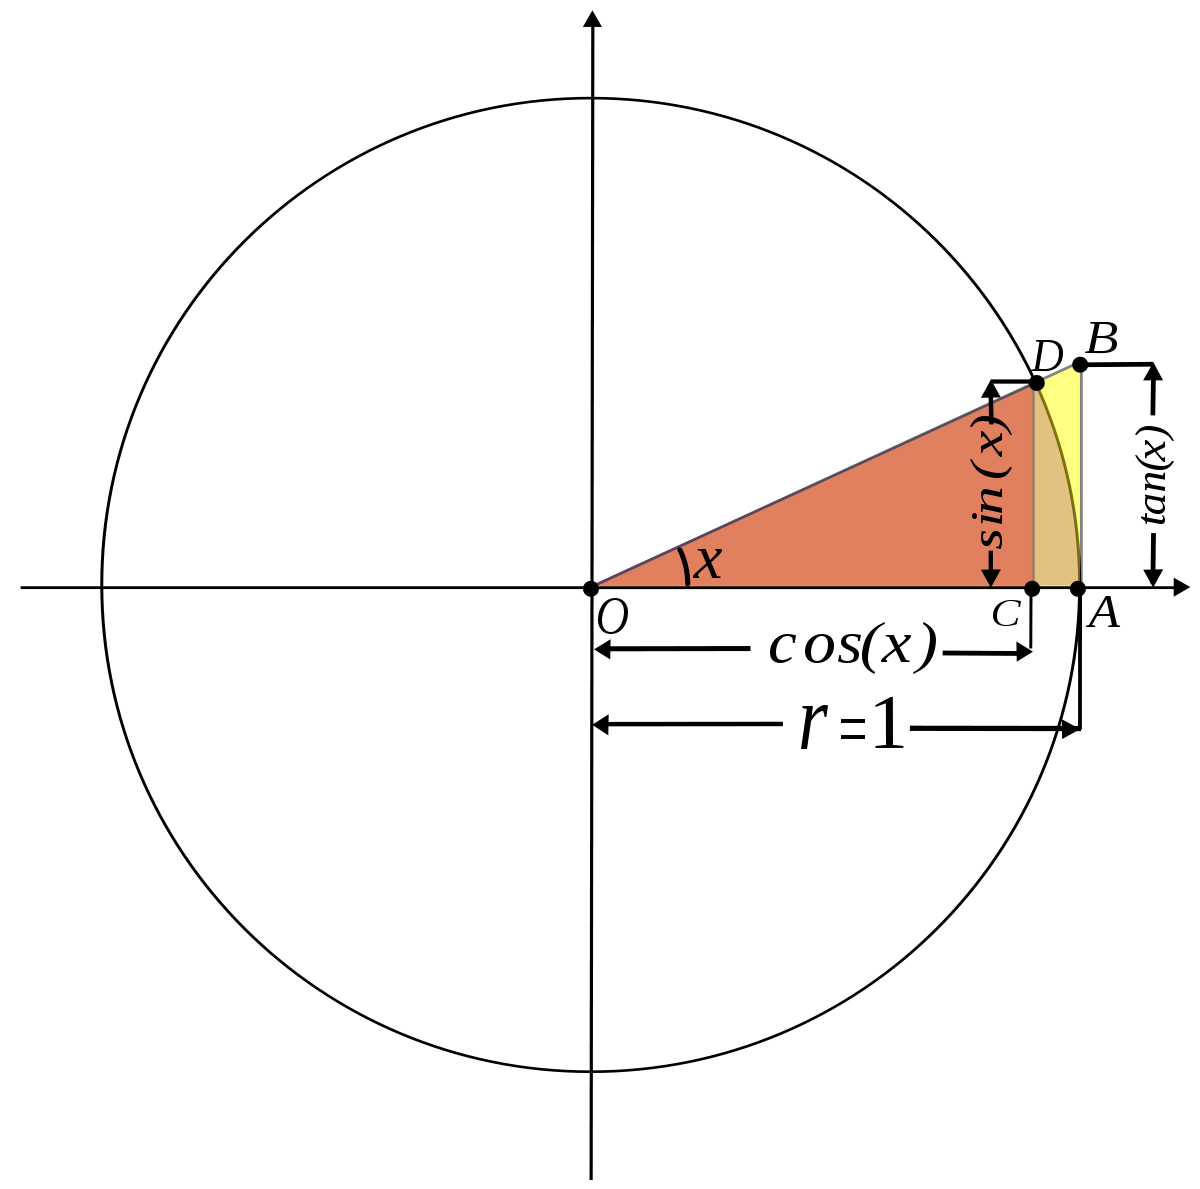
\includegraphics[width=0.35\textwidth]{circ_gon}
        \end{center}
        \[
            \cos:\mathbb{R} \rightarrow [-1,1]    
        \]
        \[
            \alpha \mapsto x_{p}    
        \]
        \[
            \sin:\mathbb{R} \rightarrow [-1,1]    
        \]
        \[
            \alpha \mapsto y_{p}    
        \]
        \subsubsection*{Proprietà}
            \begin{Large}
                \begin{itemize}
                    \item $\sin{(- \alpha)} = - \sin{\alpha}$
                    \item $\sin{(\pi - \alpha)} = \sin{\alpha}$
                    \item $\cos{(- \alpha)} = \cos{\alpha}$
                    \item $\cos{(\pi - \alpha)} = - \cos{\alpha}$
                    \item $|\sin{\alpha}| \leq 1, |\cos{\alpha}| \leq q$
                    \item $\cos$ è una funzione dispari, $\sin$ è una funzione pari
                    \item Dal teorema di pitagora: $\cos^{2}{\alpha} + \sin^{2}{alpha} = 1$
                \end{itemize}
            \end{Large}
        \subsubsection*{Formule}
            Siano $x_{1}, x_{2} \in \mathbb{R}\ \forall\ x_{1},x_{2} \in \mathbb{R}$
            \begin{Large}
                \begin{itemize}
                    \item $\cos{(x_{1} + x_{2})} = \cos{x_{1}} \cdot \cos{x_{2}} - \sin{x_{1} \cdot \sin{x_{2}}}$
                    \item $\sin{(x_{1} + x_{2})} = \sin{x_{1}} \cdot \cos{x_{2}} + \cos{x_{1} \cdot \sin{x_{2}}}$
                    \item $\cos{(2x)} = \cos^{2}{x} - \sin^{2}{x}$
                    \item $\sin{(2x)} = 2\sin{x}\cos{x}$
                    \item $|\cos{\frac{x}{2}}| = \sqrt{\frac{1 + \cos{x}}{2}}$
                    \item $|\sin{\frac{x}{2}}| = \sqrt{\frac{1 - \cos{x}}{2}}$
                \end{itemize}
            \end{Large}
    \subsubsection{Tangente}
        Sia $U$ una circonferenza goniometrica
        \begin{Large}
            \[
                \tan:\mathbb{R} \setminus \{\frac{\pi}{2} + k\pi, k \in \mathbb{Z}\} \rightarrow \mathbb{R}
            \]
            \[
                \alpha \mapsto y_{Q}    
            \]
        \end{Large}
        \begin{center}
            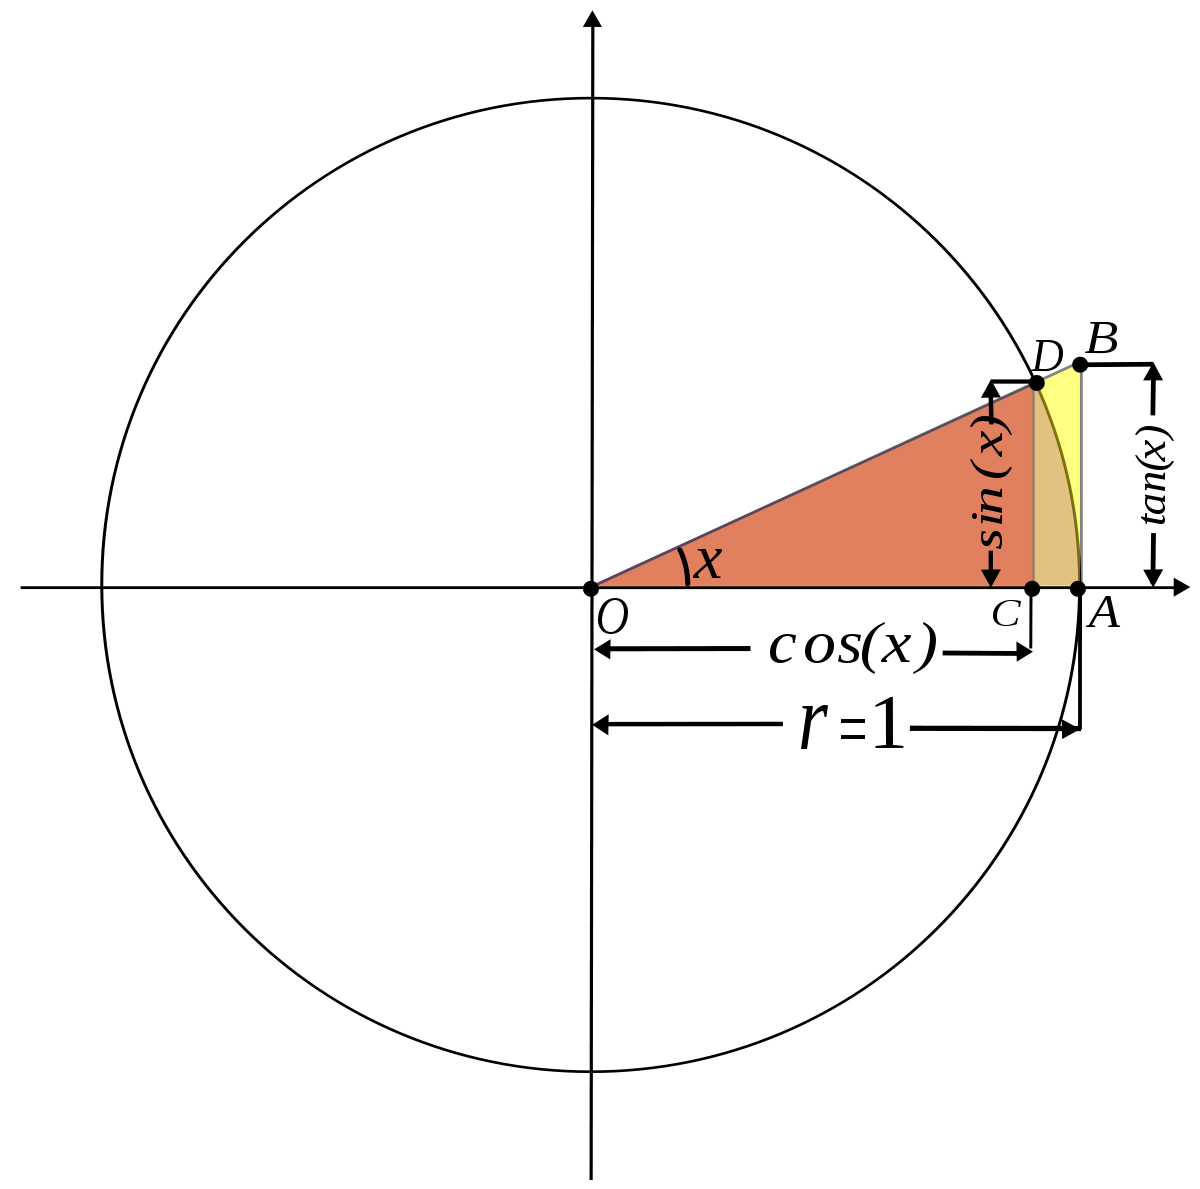
\includegraphics[width=0.35\textwidth]{circ_gon}
        \end{center}
        I triangoli $O\overset{\triangle}{P}H$ e $O\overset{\triangle}{Q}H$ sono simili, quindi:
        \[
            \frac{QK}{OK} = \frac{PH}{OH} \Rightarrow \frac{\tan{\alpha}}{1} = \frac{\sin{\alpha}}{\cos{\alpha}} \Rightarrow \tan{\alpha} = \frac{\sin{\alpha}}{\cos{\alpha}}    
        \]
        $\tan$ è periodica di periodo $\pi: \tan{(\alpha + \pi)} = \tan{\alpha}$. Dato che $\tan{\alpha}$ è una funzione dispari, e vista 
        la sua periodicità, è sufficiente studiarla solo nell'intervallo $[0, \frac{\pi}{2}[$.
        Analogamente, $cotan{\alpha} = \frac{\cos{\alpha}}{\sin{alpha}}$ (la retta è parallela all'asse $y$, passante per $(0,1)$ e si considera $x_{Q}$).
            
